% Copyright 2004 by Till Tantau <tantau@users.sourceforge.net>.
%
% In principle, this file can be redistributed and/or modified under
% the terms of the GNU Public License, version 2.
%
% However, this file is supposed to be a template to be modified
% for your own needs. For this reason, if you use this file as a
% template and not specifically distribute it as part of a another
% package/program, I grant the extra permission to freely copy and
% modify this file as you see fit and even to delete this copyright
% notice. 

\documentclass{beamer}
\usetheme{default}


\title{Speaker recognition using deep neural networks}



\author{Bajibabu Bollepalli}

\institute[Aalto University] % (optional, but mostly needed)
{
  Department of Signal Processing and Acoustics\\
  Aalto University
  }
% - Keep it simple, no one is interested in your street address.

\date{June 14, 2016}

\subject{Speaker recognition using DNNs}
% This is only inserted into the PDF information catalog. Can be left
% out. 

% Let's get started
\begin{document}

\begin{frame}
  \titlepage
\end{frame}

\begin{frame}{Outline}
  %\tableofcontents
  % You might wish to add the option [pausesections]
  \begin{itemize}
      \item{Renaissance of neural networks}
      \item{DNNs role in speaker recognition (SR)}
      \item{Extraction of i-vectors in standard SR framework}
      \item{i-vector extraction using DNNs}
      \item{Results}
      \item{Pros and cons using DNNs in SR}
      \item{Other strategies}
      \item{References}
  \end{itemize}
\end{frame}

%%%%%%%%%%%%%%%%%%%%%%%%%%%%%%%%%%%%%%%%%%%%%%%%%%%%%%%%%%%%%%%%
\begin{frame}{Renaissance of neural networks -- Deep Neural Networks (DNNs)}
\begin{itemize}
    \item{ Deep learning's successes can be explained by three factors:
  \begin{enumerate}
      \item Advances in computer hardware and software (e.g. GPUs)
      \item Abundance of data
      \item Complex models with massive number of parameters, even if they are unidentifiable and uninterpretable
  \end{enumerate}}
  
  \item
  DNN's success in ASR~\cite{Hinton2012} draws attention in speech research community
  \begin{itemize}
     \item{Outperformed the Gaussian Mixture Models in acoustic modelling}
      \item { Appearance of "deep" keyword in the proceedings of \textbf{ICASSP}-- 2011: \alert{13}, 2012: \alert{18}, 2013*: \alert{61}, 2014: 
      \alert{102}, 2015: \alert{111}, 2016: \alert{149}}
  \end{itemize}
\end{itemize}
\end{frame}

%%%%%%%%%%%%%%%%%%%%%%%%%%%%%%%%%%%%%%%%%%%%%%%%%%%%%%%%%%%%%%%%
\begin{frame}{DNNs role in speaker recognition (SR)}
  DNNs are employed in two ways in SR
  \begin{enumerate}
      \item \textbf{Direct} way~\cite{Variani2014}
            \begin{itemize}
              \item{A DNN is trained as a classifier for the intended recognition task directly to discriminate between speakers for SR}
            \end{itemize}
       \item \textbf{Indirect} way~\cite{Yun_Lei2014}
       \begin{itemize}
           \item{A DNN is possibly trained for a different purpose to extract data that is then used to train a secondary classifier for the intended recognition task}
           \item{Extract frame-level features or accumulate multi-modal statistics}
       \end{itemize}
  \end{enumerate}
  
  Most of the exist studies applied DNNs in indirect way. Thus the focus of this presentation is on the same.
\end{frame}

\begin{frame}{DNNs in indirect way}
 \begin{figure}
      \centering
      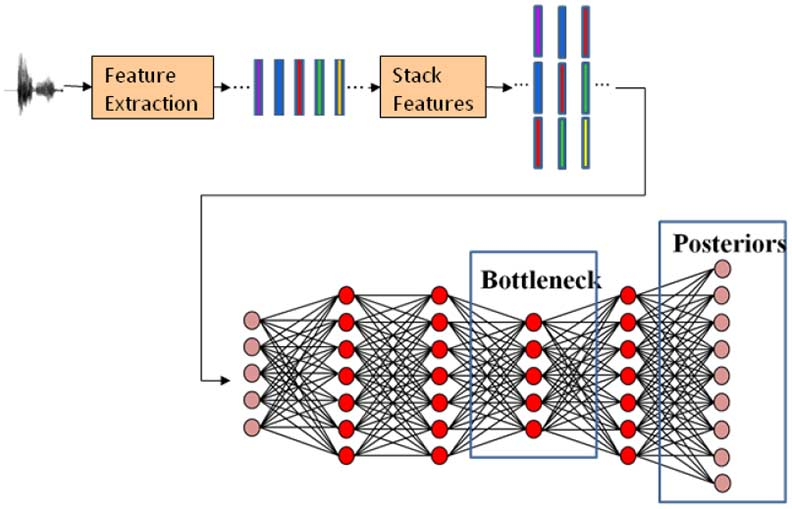
\includegraphics[width=9cm, height=5cm]{figures/indirect_dnns}
      \caption{Example of DNN architecture~\cite{Richardson2015}.}
      \label{fig:dnn_example}
  \end{figure}
 DNNs are used to extract frame-level bottleneck and/or posterior features which further processed in later steps.
\end{frame}

%%%%%%%%%%%%%%%%%%%%%%%%%%%%%%%%%%%%%%%%%%%%%%%%%%%%%%%%%%%%%%%%
\begin{frame}{A typical speaker recognition system}
  \begin{figure}
      \centering
      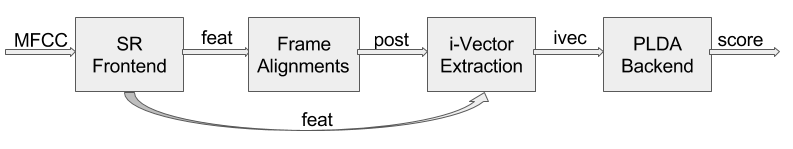
\includegraphics[width=10cm, height=2cm]{figures/SR_blockdiagram.png}
      \vspace{-4pt}
      \caption{Block Diagram of a typical speaker recognition system.}
      \label{fig:blck_sr}
  \end{figure}
  \vspace{-15pt}
  \begin{itemize}
  
  \item{ In frontend:
  \begin{itemize}
      \item VAD; Mean-variance normalization
      \item Append delta and delta-delta features
  \end{itemize}
  }
  
   \item{In frame alignments:
  \begin{itemize}
      \item Estimate posteriors for each frame based on an assumed model
      \item Normally a multi-variate Gaussian Model is used
  \end{itemize}
  }
  
   \item{In i-vector extraction:
  \begin{itemize}
      \item Estimate total variability matrix with posteriors and SR features
  \end{itemize}
  }
  
   \item{In backend:
  \begin{itemize}
      \item Mean and length normalization on i-vectors
      \item Compute similarity score between i-vectors by Probabilistic Linear Discriminant Analysis (PLDA)
  \end{itemize}
  }
   \end{itemize}
\end{frame}
%%%%%%%%%%%%%%%%%%%%%%%%%%%%%%%%%%%%%%%%%%%%%%%%%%%%%%%%%%%%%%%%

\begin{frame}{i-vector extraction}
\begin{figure}
      \centering
      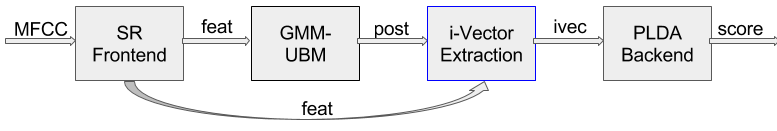
\includegraphics[width=10cm, height=2cm]{figures/ivec_blockdiagram.png}
      \vspace{-4pt}
      \caption{Block Diagram of GMM-UBM speaker recognition system.}
      \label{fig:gmm_ivec}
  \end{figure}
  \vspace{-15pt}
  \begin{itemize}
  \item {
    Represent a full utterance with a low dimensional vector
    \begin{itemize}
        \item E.g., 300x60 $\rightarrow$ 200 dimensional vector
    \end{itemize}
  }
  \item Retain both speaker- and channel-dependent information
  \item Suppose $\mathbf{x}$ is a given speech utterance and it contains $T$ feature vectors $(\mathbf{x}_1, \mathbf{x}_2,...,\mathbf{x}_T)$.
    \begin{itemize}
        \item $\mathbf{x}_t$ $\sim$ p($\mathbf{x}$, $\theta$)
        \item Following stats are needed to extract i-vector
        \begin{equation} \label{eq1}
         \begin{split}
           \gamma_{t}^{(\theta)} &= p(\theta|{\bf x}_t)             \quad \text{(frame posterior)} \\
            N_x^{(\theta)} &= \sum_t \gamma_{t}^{(\theta)}              \quad \text{(zero order statistics)} \\
            F_x^{(\theta)} &= \sum_t \gamma_{t}^{(\theta)} {\bf x}_t \quad \text{(first order statistics)}
	\end{split}
	\end{equation}
    \end{itemize}
  \end{itemize}
\end{frame}
%%%%%%%%%%%%%%%%%%%%%%%%%%%%%%%%%%%%%%%%%%%%%%%%%%%%%%%%%%%%%%%%

\begin{frame}{Frame alignments with GMM-UBM}
\begin{figure}
      \centering
      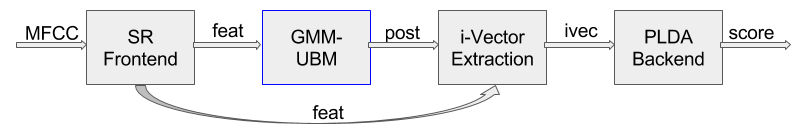
\includegraphics[width=10cm, height=2cm]{figures/UBM_blockdiagram.png}
      \vspace{-4pt}
      \caption{Block Diagram of GMM-UBM speaker recognition system.}
      \label{fig:gmm_ivec1}
  \end{figure}
  \vspace{-15pt}
\begin{block}{GMM-UBM}
\begin{itemize}
    \item Gaussian Mixture Model - Universal Background Model
    \item Typically contain 1024 or 2048 Gaussians
    \item Trained on tens or hundreds hours of speech from a large number of speakers
    \item Gender dependent or independent
    \item EM algorithm is used to estimate the GMM parameters
    \item Generally defines the speaker manifold
\end{itemize}
\end{block}
\end{frame}
%
%%%%%%%%%%%%%%%%%%%%%%%%%%%%%%%%%%%%%%%%%%%%%%%%%%%%%%%%%%%%%%%%
\begin{frame}{GMM-UBM based i-vector extraction}
\begin{figure}
      \centering
      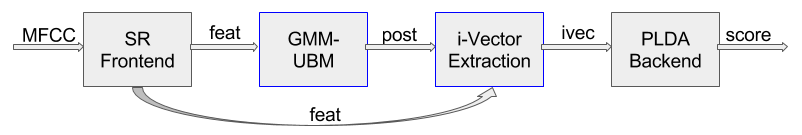
\includegraphics[width=10cm, height=2cm]{figures/UBM_ivec_blockdiagram.png}
      \vspace{-4pt}
      \caption{Block Diagram of GMM-UBM speaker recognition system.}
      \label{fig:gmm_ivec2}
  \end{figure}
  \vspace{-15pt}
  \begin{itemize}
  \item { In this model
    \begin{equation}
     \mathbf{x}_t \sim \sum_{k=1}^{K} \gamma_{t}^{(k)} N( \boldsymbol{\mu}_k + \mathbf{T}_k\boldsymbol{\omega}, \mathbf{\Sigma}_k)
   \end{equation}
    \begin{itemize}
        \item  $K$ is the number of Gaussians
        \item  $\boldsymbol{\mu}_k$ and $\mathbf{\Sigma}_k$ are mean and covariance of $k$-th Gaussian in UBM
        \item $\mathbf{T}_k$ is a low-rank rectangular matrix also called as total variability matrix
        \item $\boldsymbol{\omega}$ is a latent-variable drawn from a standard normal distribution $N(0,I)$
    \end{itemize} }
    \item The i-vector $\boldsymbol{\phi_x}$ of the utterance $\mathbf{x}$ is the maximum a posterior (MAP) point estimate of the latent vector $\boldsymbol{\omega}$.
  \end{itemize}
\end{frame}
%%%%%%%%%%%%%%%%%%%%%%%%%%%%%%%%%%%%%%%%%%%%%%%%%%%%%%%%%%%%%%%%

\begin{frame}{DNN based i-vector extraction}
  \begin{figure}
      \centering
      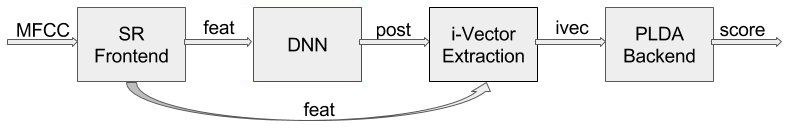
\includegraphics[width=10cm, height=2cm]{figures/DNN_ivec_blockdiagram.png}
      \vspace{-4pt}
      \caption{Block Diagram of DNN based speaker recognition system.}
      \label{fig:dnn_ivec}
  \end{figure}
  \vspace{-15pt}
 \begin{block}{DNN}
  \begin{itemize}
    \item Typically the DNN is trained for ASR task
    \item Inputs are ASR specific features and outputs are senones (tied triphone states)
    \item Need a transcribed data for training (supervision)
    \item No standard architecture settings
 \end{itemize}
 \end{block}
\end{frame}
%%%%%%%%%%%%%%%%%%%%%%%%%%%%%%%%%%%%%%%%%%%%%%%%%%%%%%%%%%%%%%%%

\begin{frame}{Bottleneck (BN) features based i-vector extraction}
\begin{figure}
      \centering
      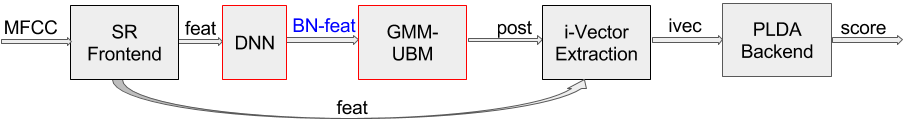
\includegraphics[width=10cm, height=2cm]{figures/BN_ivec_blockdiagram.png}
      \vspace{-4pt}
      \caption{Block Diagram of BN-UBM based speaker recognition system.}
      \label{fig:bn_ivec}
  \end{figure}
  \vspace{-15pt}
\begin{itemize}
    %\item We can use the activations of one of the DNN's hidden layers as feature vector
    \item Typically BN layer has fewer nodes then input layer
    \item BN layer with linear activation is very much like a PCA or LDA
    \item Extract using the same DNN trained for ASR task
    \item A GMM-UBM is trained with BN features to get frame alignments
    \item Have the tendency to suppress the "unimportant" speaker related information
    \item The BN features trained with GMM can depict the phonetic space more accurately
\end{itemize}
\end{frame}
%%%%%%%%%%%%%%%%%%%%%%%%%%%%%%%%%%%%%%%%%%%%%%%%%%%%%%%%%%%%%%%%

\begin{frame}{Results}
\begin{table}[]
    \centering
    \begin{tabular}{|c|c|c|c|}
      \hline
       \textbf{System}  & \textbf{Database} & \textbf{EER (\%)} & \textbf{Rel. Imp (\%)} \\ \hline
        UBM-EM(4096) & NIST SRE'12 C2 & 1.81 & - \alert{\cite{Yun_Lei2014}} \\
        DNN(3450)    & "              & 1.39 & 23  \\ \hline
        UBM-EM(4096) & NIST SRE'12 C5 & 2.55 & - \alert{\cite{Yun_Lei2014}}\\ 
        DNN(3450)    & "              & 1.92 & 25\\ \hline
        UBM-EM(2048) & NIST SRE'10 C5 & 2.91 & - \alert{\cite{Yao2015}}\\
        DNN(2227)    & "              & 2.58 & 11  \\
        BN-UBM(2227) &  "             & 2.28 & 22  \\ \hline
    \end{tabular}
    \caption{Equal error-rate (EER) comparison of gender dependent models on differnt datasets.}
    \label{tab:my_label}
For my course project, I am replicating the demo shared in Kaldi "egs/sre10/v2/"
\end{table}
  
\end{frame}

%%%%%%%%%%%%%%%%%%%%%%%%%%%%%%%%%%%%%%%%%%%%%%%%%%%%%%%%%%%%%%%%
\begin{frame} {Pros and cons}
\begin{block}{Pros}
\begin{itemize}
    \item The UBM-defined classes and posteriors have no inherent meaning
    \item Each Gaussian in UBM may cover more than one phoneme or part of phoneme
    \item DNNs success in ASR i.e improvements in word error rate compared to GMMs
    \item DNNs trained with senones capture the speaker specific pronunciations
\end{itemize}
\end{block}
\begin{block}{Cons}
\begin{itemize}
    \item Senones are dependent on language
    \item Need huge amount of computational resources
    \item The recognition performance greatly depends on the data used for training the DNN
\end{itemize}
\end{block}
\end{frame}
%%%%%%%%%%%%%%%%%%%%%%%%%%%%%%%%%%%%%%%%%%%%%%%%%%%%%%%%%%%%%%%%

\begin{frame}{Other strategies}
\begin{itemize}
    \item Convolutional neural networks (CNN)~\cite{Mitchell2014}
    \begin{itemize}
        \item{Showed better performance in noisy conditions in both ASR and SR}
    \end{itemize}
    \item Time delay neural networks (TDNN)~\cite{Synder2015}
    \begin{itemize}
        \item{It is an extended MLP architecture}
        \item{Uses sequential information in speech}
        %\item{}
    \end{itemize}
   
    \item May be recurrent neural newtorks (RNNs)?
    \begin{itemize}
        \item{No papers yet}
    \end{itemize}
    \item{Can we use autoencoders to extract BN features?}
\end{itemize}
\end{frame}

%%%%%%%%%%%%%%%%%%%%%%%%%%%%%%%%%%%%%%%%%%%%%%%%%%%%%%%%%%%%%%%%

% All of the following is optional and typically not needed. 
\appendix
\section<presentation>*{\appendixname}
\subsection<presentation>*{References}

\begin{frame}[allowframebreaks]
  \frametitle<presentation>{References}
    
  \begin{thebibliography}{8}
    
   
 \beamertemplatearticlebibitems
  % Followed by interesting articles. Keep the list short. 
 \bibitem{Hinton2012}
 Geoffrey  Hinton, et al. 
 \newblock{Deep neural networks for acoustic modeling in speech recognition: The shared views of four research groups.}
 \newblock{\em IEEE Signal Processing Magazine}, vol. 29.6, pp. 82-97, 2012.
 
 \bibitem{Variani2014}
  Ehsan Variani, Xin Lei, Erik McDermott, Ignacio Lopez Moreno, and Javier Gonzalez-Dominguez. 
  \newblock{Deep neural networks for small footprint text-dependent speaker verification.}
  \newblock{\em ICASSP}, pp. 4052-4056, 2014.

  \bibitem{Yun_Lei2014}
  Yun Lei, Nicolas Scheffer, Luciana Ferrer, and Mitchell McLaren.
  \newblock{A novel scheme for speaker recognition using a phonetically-aware deep neural network.}
  \newblock{\em ICASSP}, pp. 1695-1699, 2014.
 
  \bibitem{Richardson2015}
  Fred Richardson, Douglas Reynolds, and Najim Dehak.
  \newblock{Deep neural network approaches to speaker and language recognition.}
  \newblock{\em IEEE Signal Processing Letters}, vol. 22.10, pp. 1671-1675, 2015.
 
  \bibitem{Yao2015}
  Yao Tian, Meng Cai, Liang He, Jia Liu.
  \newblock{Investigation of bottleneck features and multilingual deep neural networks for speaker verification.}
  \newblock{\em Interspeech}, Dresden, Germany, pp. 1151-1155, 2015.
  
  \bibitem{Mitchell2014}
  Mitchell McLaren, Yun Lei, Nicolas Scheffer, Luciana Ferrer
  \newblock{Application of convolutional neural networks to speaker recognition in noisy conditions.}
  \newblock{\em Interspeech}, Singapore, pp. 686-690 2014.
  
  \bibitem{Synder2015}
  David Snyder, Daniel Garcia-Romero and Daniel Povey.
  \newblock{Time delay deep neural network-based universal background models for speaker recognition.}
  \newblock{\em IEEE ASRU},  pp. 92-97, 2015.
  
\end{thebibliography}
\end{frame}

\end{document}


